%%%%%%%%%%%%%%%%%%%%%%%%%%%%%%%%%%%%%%%%%%%%%%%%%%%%%%%%%%%
% --------------------------------------------------------
% Rho
% LaTeX Template
% Version 2.1.1 (01/09/2024)
%
% Authors: 
% Guillermo Jimenez (memo.notess1@gmail.com)
% Eduardo Gracidas (eduardo.gracidas29@gmail.com)
% 
% License:
% Creative Commons CC BY 4.0
% --------------------------------------------------------
%%%%%%%%%%%%%%%%%%%%%%%%%%%%%%%%%%%%%%%%%%%%%%%%%%%%%%%%%%%

\documentclass[10pt,a4paper,twoside]{rho-class/rho}
\usepackage[english]{babel}

%% Spanish babel recomendation
% \usepackage[spanish,es-nodecimaldot,es-noindentfirst]{babel}

\setbool{rho-abstract}{true} % Set false to hide the abstract
\setbool{corres-info}{true} % Set false to hide the corresponding author section

%----------------------------------------------------------
% TITLE
%----------------------------------------------------------

%\journalname{Molecular Ecology}
\title{Genome-Wide Analysis Reveals Altitude-Associated Divergence in a Colour-Polymorphic Insect}
%----------------------------------------------------------
% AUTHORS AND AFFILIATIONS
%----------------------------------------------------------

\author{}

%----------------------------------------------------------

\affil{}

%----------------------------------------------------------
% DATES
%----------------------------------------------------------

\dates{This manuscript was compiled on December 23, 2025}

%----------------------------------------------------------
% FOOTER INFORMATION
%----------------------------------------------------------

\leadauthor{}
\smalltitle{Altitude-Associated Genomic Divergence}

%----------------------------------------------------------
% ARTICLE INFORMATION
%----------------------------------------------------------

\corres{}
\email{}

%----------------------------------------------------------
% ABSTRACT
%----------------------------------------------------------

\begin{abstract}
    Environmental gradients provide powerful natural experiments for understanding how selection and gene flow interact to shape genomic and phenotypic variation. However, the genetic basis of adaptation across steep altitudinal clines remains poorly resolved, particularly in systems with high connectivity. We studied the montane bush cricket Isophya rizeensis, which exhibits a discrete male colour polymorphism along a continuous 450–2,300 m elevational transect in the Fırtına Valley (Türkiye), with a sharp transition between dark and pale morphs near mid‐elevations. Using genome-wide RAD sequencing of 71 individuals, we identified over 92,000 SNPs and detected weak overall population structure consistent with substantial connectivity along the gradient. Despite this, putatively adaptive loci showed markedly stronger spatial differentiation than neutral loci. Genome-wide association analyses identified 101 SNPs significantly associated with altitude, exhibiting reciprocal allele-frequency shifts and steep, narrow clines concentrated over short elevational distances. Discriminant analyses further revealed three loci of large effect that strongly differentiate colour morphs and are tightly linked to elevation. Together, these results indicate that spatially varying selection can maintain discrete phenotypic polymorphism and localized genomic divergence despite high connectivity. Our findings provide empirical support for clinal models of local adaptation under gene flow and highlights how environmental heterogeneity structures adaptive genetic variation in montane ecosystems.
\end{abstract}

%----------------------------------------------------------

\keywords{Clinal variation, Local adaptation, Spatially varying selection, Genotype--phenotype association, RAD sequencing, Non-model insect, \textit{Isophya rizeensis}}

%----------------------------------------------------------

\begin{document}
	
    \maketitle
    \thispagestyle{firststyle}
    % \tableofcontents
    \linenumbers

%----------------------------------------------------------

\section{Introduction}

    Understanding how environmental gradients shape genetic and phenotypic variation is a central question in evolutionary ecology. Altitudinal gradients, in particular, serve as powerful natural laboratories for examining the interplay between gene flow, selection, and drift across steep and predictable environmental transitions (\cite{Wogan2018}; \cite{Kelly2019}). Such gradients impose structured ecological variation (including shifts in temperature, humidity, oxygen availability, and habitat structure) that can promote local adaptation by favoring different alleles or traits at different elevations (\cite{Muir2014}). Investigating how genomic and phenotypic diversity align with these gradients offers insight into the mechanisms underlying population differentiation and adaptation (\cite{Merilä2014}; \cite{Waldvogel2020}).

    Altitudinal gradients are especially informative because they generate sharp environmental transitions over short geographic distances, which can reduce gene flow and strengthen divergent selection (\cite{Chown2003}; \cite{Flatt2016}). The resulting spatial structuring may amplify isolation by distance (IBD), whereby genetic similarity decreases with geographic distance (\cite{Orsini2013}). At the same time, strong selective pressures such as thermal variation, hypoxia, and vegetation structure can drive adaptive divergence across elevation (\cite{Sexton2014}; \cite{Stankowski2017}; \cite{Bradburd2019}). Combined with genotype--environment association approaches, altitudinal clines have become a powerful framework for identifying loci under spatially varying selection (\cite{Hancock2011}; \cite{Slatyer2014}; \cite{Pluess2016}), providing insight into how selection acts across heterogeneous landscapes (\cite{Mayekar2022}; \cite{Tyrmi2020}; \cite{Soliani2020}).
    
    One well-documented axis of altitudinal divergence in ectotherms is colour polymorphism. In insects, colour traits are frequently linked to thermoregulation, camouflage, and ecological specialization, influencing survival and fitness (\cite{Forsman2008}; \cite{Zeuss2014}; \cite{Kozlov2022}). One widely reported pattern is classical thermal melanism, which predicts darker phenotypes at cooler, higher elevations due to increased solar absorption (\cite{CLUSELLATRULLAS2007}; \cite{Clusella-Trullas2020}). However, many systems deviate from this expectation, indicating that additional ecological factors such as habitat structure, solar exposure, and predation also shape colour evolution (\cite{Karlsson2008}; \cite{Goodman2021}). Colour polymorphism can also expand niche breadth by allowing different morphs to perform optimally under distinct environmental conditions, thereby enhancing ecological resilience and population persistence (\cite{Forsman2008}; \cite{Wennersten2009}; \cite{Kozlov2022}). Therefore, understanding the genetic basis of such variation is key to linking phenotypic divergence to underlying evolutionary processes (\cite{Forsman2016}; \cite{McLean2014}).
    
    The montane bush cricket \textit{Isophya rizeensis} (Orthoptera: Tettigoniidae: Phaneropterinae: Barbitistini) provides an exceptional system for studying altitudinal adaptation (\cite{SEVGILI2003}). This species is narrowly endemic to the Fırtına Valley and neighboring valleys of the Pontic Mountains, where its distribution is highly fragmented and largely restricted to isolated subalpine habitats above approximately 1{,}600~m. Notably, the Fırtına Valley is the only known location where \textit{I.~rizeensis} occurs continuously from lowland habitats ($\sim$300~m) to elevations exceeding 2{,}300~m, forming a complete elevational transect (Figure~1).
    
    Along this gradient, vegetation and habitat structure change predictably: densely shaded Colchic broadleaf and boxwood forests dominate lower elevations ($<$900~m), cooler mixed beech--spruce--fir forests occur at mid-elevations, and open, sparsely vegetated subalpine meadows characterize elevations above $\sim$1{,}800~m, where solar exposure is high and thermal conditions are more extreme (\cite{Karacaoglu2014}). Within this environmental mosaic, males exhibit a striking and spatially structured dorsal colour polymorphism. Dark males dominate lower elevations (approximately 350--1{,}000~m), while pale morphs occur at higher elevations (1{,}100--2{,}300~m), with populations typically monomorphic and a sharp transition between morphs near 1{,}100~m (\cite{SaglamCaglar2005}; \cite{SaglamCaglar2007Isophya}; \cite{Çağlar2014}). Females also vary in colouration, but this variation is limited to subtle shades of green and lacks the discrete black--green divergence observed in males (\cite{SEVGILI2003}; \cite{SaglamCaglar2005}).
    
    This distribution contrasts with expectations under classical thermal melanism. Physiological data in \textit{I. rizeensis} indicate that darker males warm more rapidly and attain higher body temperatures than paler individuals, a trait that may be maladaptive in open subalpine habitats where surface temperatures frequently exceed 40~$^\circ$C due to intense solar radiation. Under such conditions, paler colouration may reduce overheating risk and thus confer a selective advantage (\cite{Kuyucu2016}). Despite these ecological observations, the genomic architecture underlying this colour polymorphism and its relationship with elevation remain poorly understood. In particular, it is unclear whether phenotypic divergence reflects local adaptation or is shaped primarily by neutral processes.
 
    Here, we investigate the genomic basis of altitudinal colour divergence in \textit{I.~rizeensis} by integrating genome-wide RAD sequencing with population genetic and genotype--phenotype association analyses. Focusing on male phenotypes, which exhibit discrete and ecologically well-characterized colour morphs (\cite{Çağlar2014}), we aim to: (1) characterize population structure and connectivity along an elevational gradient; (2) disentangle neutral from adaptive genetic differentiation; and (3) identify loci associated with both altitude and colour polymorphism. By coupling genomic data with elevation and phenotypic gradients, our study provides insight into how spatially varying selection can maintain adaptive genetic variation and discrete phenotypes across a heterogeneous montane landscape.

\section{Materials and Methods}

    \subsection{Sample Collection and Sequencing}

        Male specimens were collected between June and August 2006 from 11 sites spanning an altitudinal gradient from 450 to 2{,}300~m in the Fırtına Valley (Figure~1) using sweep netting and categorized by dorsal colouration following \cite{Çağlar2014}. Genomic DNA was extracted from hind femora using the \textsc{E.Z.N.A.}® Insect DNA Kit (Omega Bio-Tek) according to the manufacturer’s protocol. Genome-wide variation was characterized using Restriction site--Associated DNA sequencing (RAD-seq). Paired-end RAD libraries were prepared using the \textit{PstI} restriction enzyme following \cite{Ali2016} (see \textbf{Supplementary Information: RAD Library Preparation} for details). Libraries were sequenced on an Illumina HiSeq4000 platform at the UC Davis Genome Center to an average depth of $\sim$10$\times$. In total, 75 \textit{I.~rizeensis} individuals were sequenced, with 5--7 individuals per sampling site.

    \subsection{Alignment and Filtering}

        Because no reference genome is available for \textit{I.~rizeensis} or any closely related species, we generated a de novo RAD reference following the procedure described in \cite{SağlamMolEcol2016} (see \textbf{Supplementary Information: De-novo RAD locus discovery and extension} for details). Raw reads were aligned to RAD contigs using \textsc{bwa-mem} (\cite{Li2010}; \cite{Li2013}). Alignments were converted to coordinate-sorted \textsc{BAM} files with \textsc{samtools} (\cite{Danecek2021}), and duplicate reads were marked using \textsc{Picard}. Paralogous RAD-contigs were identified with \textsc{ngsParalog} (\cite{Linderoth2018}) and excluded from downstream analyses.

    \subsection{SNP Discovery and Genotyping}

        SNP discovery was performed in \textsc{ANGSD} (\cite{Korneliussen2014}) by determining genotype likelihoods (\texttt{-GL 1}), major and minor alleles (\texttt{-doMajorMinor 1}), minor allele frequencies (\texttt{-doMaf 1}), and generation of \textsc{BCF/VCF} files (\texttt{-doBcf 1}). SNPs were filtered to retain sites with MAF $\geq$ 0.05 (\texttt{-minMaf 0.05}), minimum base quality 20 (\texttt{-minQ 20}), minimum mapping quality 10 (\texttt{-minMapQ 10}), posterior genotype probability $\geq$ 0.85 (\texttt{-postCutoff 0.85}), and proper read pairing (\texttt{-only\_proper\_pairs 1}).  Sites were further required to be polymorphic based on likelihood tests ($P < 10^{-12}$), have a mean per-individual depth $\geq$6$\times$, and be present in at least 50\% of individuals per population.

    \subsection{Population Genetic Structure}

        Population structure was assessed using principal component analysis (PCA) based on genotype likelihoods. A genetic covariance matrix was estimated in \textsc{PCAngsd} (\cite{Meisner2018}) and subjected to eigen decomposition in \textit{R} (v4.2.0; \cite{R2024}). The first two principal components were visualized to summarize major axes of genetic variation.

        Individual ancestry proportions were inferred using \textsc{NgsAdmix} (\cite{Skotte2013}), with K values ranging from 2 to 5 and ten independent runs per K. To reduce overfitting and spurious clustering under weak or continuous population structure, admixture inference was restricted to a maximum K of 5 (\cite{Lawson2018}). The most likely number of clusters was evaluated using the $\Delta K$ method (\cite{Evanno2005}), and admixture proportions were visualized in \textit{R}.

    \subsection{Genetic Differentiation and Isolation by Distance}

        Genome-wide genetic differentiation among sampling sites was quantified using pairwise $F_{ST}$ estimated in \textsc{ANGSD} under a likelihood-based framework. Site allele frequency likelihoods were calculated for each population pair, and joint two-dimensional site frequency spectra (2D-SFS) were inferred using \texttt{realSFS}. Weighted global $F_{ST}$ values were computed using the \texttt{-whichFst 1} estimator (\cite{Nielsen2012}), which performs well with moderate sample sizes (\cite{Willing2012}). Folded SFS were well formed and consistent across elevations (Supplementary Figure~S1), indicating that estimates were not driven by elevation-dependent allelic dropout or sampling bias.

        Isolation by distance (IBD) was tested using Mantel tests comparing linearized pairwise $F_{ST}$ [$F_{ST}/(1-F_{ST})$] with Euclidean geographic distances computed in the \textsc{Geographic Distance Matrix Generator} v1.2.3 (\cite{Ersts2024}). Pearson and Spearman correlations were assessed with 999 permutations using the \texttt{vegan} package in \textit{R} (\cite{Mantel1967}; \cite{Oksanen2001}).

    \subsection{Comparing Neutral and Adaptive Genetic Variation}

        Putatively adaptive loci were identified using the \texttt{Pcadapt} framework implemented in \textsc{PCAngsd}, which detects SNPs associated with major axes of genetic variation inferred from PCA (\cite{Meisner2018}; \cite{Luu2017}). The number of significant principal components was determined using Velicer’s minimum average partial test (\cite{Shriner2011}), which supported a single axis (K = 1). SNP outliers were identified based on Mahalanobis distances of SNP loadings and assessed under a $\chi^2$ distribution, with false discovery rate correction applied (\cite{BenjaminiHochberg1995}). To exclude loci affected by inbreeding, SNPs flagged by the \texttt{--inbreedSites} and \texttt{--inbreed} procedures were removed, yielding a final dataset of 82{,}976 SNPs and a genome-wide significance threshold of $6.03 \times 10^{-7}$ ($\chi^{2} = 24.903$, $df = 1$, $\alpha = 0.05$) for identifying putatively adaptive loci.

        Genetic diversity was estimated separately for neutral and adaptive data sets using nucleotide diversity ($\theta_{\pi}$) calculated from the folded site frequency spectrum. Allele frequency likelihoods were estimated in \textsc{ANGSD} (\texttt{-doSaf 1}), and the SFS was inferred using \texttt{realSFS}. Genome-wide $\theta_{\pi}$ was computed using \texttt{thetaStat} (\texttt{-do\_stat}), incorporating both polymorphic and invariant sites per RAD locus.

        To compare spatial patterns of differentiation between neutral and adaptive loci, pairwise $F_{ST}$ matrices were estimated separately for each SNP set and evaluated for isolation by distance using Mantel tests.

    \subsection{Genetic Variation Associated with Altitude}

        Genome-wide associations with altitude were tested using score statistics (\texttt{-doAsso 2}) in \textsc{ANGSD}, applying a generalized linear model with posterior genotype probabilities as the response and altitude as a quantitative predictor (\cite{Skotte2012}).
        
        In addition to previously applied filtering criteria, SNPs were required to contain at least ten posterior observations per genotype class (\texttt{-minHigh 10}). This filter ensures that each genotype category has sufficient posterior support to yield reliable likelihood-based regression coefficients in the score test. Likelihood ratio statistics were converted to \textit{P}-values assuming a $\chi^2$ distribution with one degree of freedom, and significance was assessed using a Bonferroni correction.
        
        For loci surpassing the significance threshold, the globally defined minor allele was identified and its frequency estimated at each sampling site. Allele-frequency change across elevation was summarized using a two-slope linear model (\textit{MAF $\sim$ altitude $\times$ trend}), where \textit{trend} denotes increasing or decreasing frequency with altitude.
        
        To characterize spatial turnover in allele frequencies, one-dimensional cline models were fitted to each significant SNP using \texttt{HZAR} (\cite{Derryberry2014}). Models with free asymptotes and no tails were fitted by maximum likelihood, yielding estimates of cline center, width, and amplitude ($\Delta p$) (\cite{BartonGale1993}). Poorly constrained or extrapolated fits were excluded from further analyses.

    \subsection{Genetic Discrimination of Colour Morphs}

        Genetic discrimination between  colour morphs was assessed using Discriminant Analysis of Principal Components (DAPC) implemented in \texttt{adegenet} (v2.1.1; \cite{Jombart2008}; \cite{Jombart2011}). Genotypes were called in \textsc{ANGSD} using posterior probabilities (\texttt{-doGeno 4}, \texttt{-doPost 2}) with a cutoff of 0.85 and exported as \textsc{VCF/BCF} files. The DAPC retained principal components explaining up to 80\% of the variance, with colour morph specified as the grouping factor.

        SNP contributions to discriminant functions were clustered using the \texttt{snpzip} procedure in \texttt{adegenet}, distinguishing loci with high versus low discriminatory power. Genotype states at outlier loci were visualized as heatmaps using \texttt{ggplot2}, illustrating differences in allelic composition between dark and pale morphs.

\section{Results}

    \subsection{Robust Genome-Wide Marker Discovery in a Non-Model Insect}

        Using a de novo RAD reference assembly, we identified 224{,}187 unique RAD contigs ranging from 250 to 800~bp (mean = 324~bp). Mapping success to the reference contigs ranged from 73--83\% (mean = 77\%), with an average per-individual depth of 5--6$\times$. Detailed read counts and alignment statistics are provided in Supplementary Table~S1. Individuals with fewer than 1{,}000{,}000 aligned reads after filtering were excluded, resulting in a final dataset of 71 individuals from 11 sampling sites (Table~1). Across all sampling sites, we retained 9{,}616 polymorphic RAD contigs containing 92{,}047 high-confidence SNPs passing all filtering criteria. Mean per-individual missingness ranged from 0.12 to 0.39 across populations (Supplementary Table~S2) and was not correlated with elevation (Pearson $r = -0.396$, $p = 0.228$), indicating no systematic altitudinal bias in allelic dropout.
        
\begin{table}[ht]
\captionsetup{font=normalsize, labelfont=bf, justification=raggedright, singlelinecheck=false}
\caption{Altitude, coordinates, colour category and sample sizes of
\textit{I. rizeensis} used in this study.}
\label{tab:my-table}
\normalsize  % <-- controls table body
\begin{tabular*}{\columnwidth}{@{\extracolsep{\fill}} l l l l r}
\toprule
Altitude (m) & Latitude & Longitude & Colour & N \\
\midrule
450  & 40.9856 & 40.9646 & DARK & 7 \\
850  & 40.9406 & 40.9850 & DARK & 6 \\
900  & 40.9166 & 40.9456 & DARK & 7 \\
1000 & 40.9075 & 40.9479 & DARK & 7 \\
1100 & 40.8880 & 40.9297 & PALE & 7 \\
1200 & 40.8630 & 40.9342 & PALE & 5 \\
1300 & 40.8638 & 40.9501 & PALE & 5 \\
1900 & 40.8548 & 41.0125 & PALE & 7 \\
2000 & 40.7998 & 40.9217 & PALE & 7 \\
2100 & 40.7995 & 40.9588 & PALE & 7 \\
2300 & 40.7915 & 40.9574 & PALE & 6 \\
\bottomrule
\end{tabular*}
\end{table}

    \subsection{Weak Population Structure along the Altitudinal Gradient}

        Principal component analysis (PCA) revealed weak but continuous genetic structure along the altitudinal gradient (Figure~2A). PC1 and PC2 explained only 3.82\% and 2.08\% of the total genetic variance, respectively, indicating very shallow population structure. Individuals were broadly ordered by elevation along PC1, with partial overlap between dark and pale morphs. Variation along PC2 likely reflects stochastic or technical effects rather than biologically meaningful structure (Supplementary Figure~S2).

        Admixture analyses supported K = 2 as the optimal clustering solution (Supplementary Figure~S3). Ancestry proportions changed gradually with elevation rather than forming discrete population units (Figure~2B). This pattern persisted across higher K values (K = 3--5; Supplementary Figure~S4), consistent with continuous gene flow and weak population subdivision along the transect.

        Pairwise $F_{ST}$ values were low across the gradient (< 0.05), indicating substantial genetic connectivity among sites (Supplementary Figure~S5). Despite low overall divergence, Mantel tests revealed a strong and significant pattern of isolation by distance (IBD), with linearized $F_{ST}$ increasing with geographic distance (Pearson $r_p = 0.838$, Spearman $r_s = 0.869$, $P = 0.001$; Figure~2C).

    \subsection{Adaptive Loci Exhibit Stronger Spatial Differentiation than Neutral Variation}

        \texttt{Pcadapt} identified 1{,}113 putatively adaptive SNPs across 809 RAD-contigs and 81{,}863 neutral SNPs across 8{,}699 contigs. Genome-wide nucleotide diversity ($\theta_\pi$) was relatively high and consistent across elevations, ranging from 0.058 to 0.065 (Figure~3A; Table~S3). Neutral loci exhibited slightly higher $\theta_\pi$ than adaptive loci at all elevations, although this difference was small and statistically significant only at a subset of mid-elevation sites (900--1{,}900~m). Overall diversity patterns were similar between SNP classes.

        Genetic divergence increased with geographic distance for both adaptive and neutral loci; however, the relationship was significantly steeper for adaptive SNPs (Pearson $r = 0.91$, Spearman $r = 0.91$, $P = 0.001$) than for neutral SNPs (Pearson $r_p = 0.84$, Spearman $r_s = 0.87$, $P = 0.001$; Figure~3B). This contrast indicates stronger spatial differentiation at adaptive loci, consistent with the action of spatially varying selection  along the altitudinal gradient.

    \subsection{Altitude-Associated Loci Form Steep, Narrow Genetic Clines}

        Genome-wide association mapping using altitude as a quantitative predictor was conducted on 53{,}901 SNPs, yielding a genome-wide significance threshold of $9.28 \times 10^{-7}$ ($\alpha = 0.05$; LRT $> 24.07$). This analysis identified 101 SNPs within 75 RAD-contigs significantly associated with altitude (Table~S4), of which 73 contigs were also classified as putatively adaptive by \texttt{Pcadapt}.

       Allele-frequency changes at associated loci were bidirectional, with subsets of loci increasing or decreasing with elevation (Figure~4). A two-slope linear model explained 62\% of the variance in allele frequencies ($R^2 = 0.622$, $F_{3,1118} = 612.8$, $p < 2.2 \times 10^{-16}$), with a highly significant altitude $\times$ trend interaction confirming distinct slopes for increasing and decreasing loci (Table~S5).

        Maximum-likelihood cline models were successfully fitted for 91 of the 101 significant loci after excluding non-informative or extrapolated solutions (Table~S6). Decreasing loci exhibited narrow clines centered near mid-elevations ($\sim$1{,}100~m), whereas increasing loci showed similarly steep clines centered at higher elevations ($\sim$1{,}700~m). Median cline widths were narrow in both classes (100--200~m), and allele-frequency amplitudes were large ($\Delta p \approx 0.40$--0.45), consistent with strong spatially varying selection (Table~2).

\begin{table}[ht]
\setlength{\tabcolsep}{2pt}
\renewcommand{\arraystretch}{1.3}
\captionsetup{font=normalsize, labelfont=bf, justification=raggedright, singlelinecheck=false}
\caption{Summary of maximum-likelihood cline parameters for loci significantly
associated with altitude. Values are given as medians with interquartile ranges
(Q1--Q3) in brackets.}
\label{tab:cline_summary}
\normalsize
\resizebox{\columnwidth}{!}{%
\begin{tabular}{lcccc}
\toprule
\textbf{Trend} & \textbf{$N_\text{loci}$} & \textbf{Center [m]} &
\textbf{Width [m]} & \textbf{$\Delta p$} \\
\midrule
Decreasing & 33 & 1178 [903--1488] & 130 [87--615] & 0.47 [0.38--0.55] \\
Increasing & 58 & 1707 [1389--2028] & 196 [120--747] & 0.40 [0.33--0.53] \\
\bottomrule
\end{tabular}
}
\end{table}

    \subsection{Few Loci of Large Effect Underlie Colour Morph Differentiation}

        Discriminant analysis of principal components (DAPC) separated individuals into two groups along the first discriminant function (DF1), revealing strong genetic discrimination between dark and pale colour morphs (Figure~5A). Classification success was high (mean posterior probability = 0.97), with all pale individuals correctly assigned and 92.6\% of dark individuals correctly classified; only two dark individuals were misassigned as pale (Supplementary Figure~S6).
        
        Three loci contributed disproportionately to discrimination between morphs (Figure~5B) and displayed bimodal genotype distributions, with pale individuals nearly fixed for the major allele and dark individuals predominantly heterozygous (Figure~5C). All three loci were classified as putatively adaptive and significantly associated with altitude (Table~S4), linking colour polymorphism to altitudinal adaptation.

\section{Discussion}

    Environmental gradients provide powerful natural experiments for examining how selection, gene flow, and drift shape genomic and phenotypic variation. By integrating genome-wide, environmental, and phenotypic data, our study shows that steep altitudinal transitions can generate strong differentiation at a subset of loci despite high overall connectivity. Together, these results illustrate how spatially variable selection can maintain discrete phenotypes across a continuous montane landscape.

    \subsection{Stronger Spatial Differentiation at Adaptive Loci Despite High Connectivity}

        In systems with spatial environmental heterogeneity, distinguishing between neutral and adaptive differentiation is central to understanding selection under gene flow. Our findings show that even in landscapes with low genome-wide differentiation, subsets of putatively adaptive loci can exhibit strong divergence, particularly across steep altitudinal transitions. 

        PCA and admixture analyses revealed weak population structure and smooth changes in ancestry along the transect, consistent with high connectivity across elevations. Only the lowest and highest sites showed more homogeneous ancestry, a pattern commonly observed at ecological extremes where habitat differences intensify and dispersal declines (\cite{Byars2009}; \cite{Polato2017}; \cite{Cortázar-Chinarro2017}). Genome-wide nucleotide diversity was largely uniform across elevations, with only modest reductions at putatively adaptive loci at some mid-elevation sites, consistent with spatially varying selection under ongoing gene flow (\cite{Hoban2016}; \cite{TiganoFriesen2016}).

        Against this background of high connectivity, putatively adaptive loci exhibited substantially stronger divergence than neutral loci, with the steepest differentiation toward elevational extremes. Similar patterns have been reported across montane plants, insects, and amphibians, where strong environmental contrasts generate narrow zones of allele-frequency turnover (\cite{Byars2009}; \cite{Polato2017}; \cite{Zancolli2019}). In our system, cline analyses show that divergence at adaptive loci is spatially concentrated over short elevational distances, indicating localized allele-frequency shifts rather than broad-scale population subdivision. This pattern is consistent with selection acting across narrow environmental transition zones where multiple factors covary and change rapidly, despite continuous habitat connectivity (\cite{polechova2011}; \cite{TiganoFriesen2016}; \cite{Zancolli2019}).

        While genome-wide differentiation remained low ($F_{ST} < 0.05$), adaptive loci showed both elevated divergence and a markedly steeper isolation-by-distance pattern than neutral loci. Bidirectional allele-frequency changes across elevation further support divergent selection favoring alternate alleles in contrasting environments (\cite{White2021}; \cite{Wadgymar2022}), a pattern widely observed in clinal systems where environmental heterogeneity maintains polymorphism under gene flow (\cite{TiganoFriesen2016}; \cite{Zancolli2019}; \cite{Berdahl2015}; \cite{Forester2016}). Together, these results support a role for isolation by environment acting alongside isolation by distance in shaping genomic differentiation across the altitudinal gradient, despite pervasive gene flow (\cite{Raeymaekers2017}; \cite{Jiang2019}; \cite{Wagutu2022}; \cite{Wakamiya2023}).

    \subsection{Genotype--Phenotype Clines Support Environmentally Mediated Colour Divergence}

        Discrete phenotypes distributed along environmental gradients are a hallmark of ecologically mediated divergence. In \textit{Isophya}, three loci showed exceptionally strong discriminatory power between colour morphs: pale individuals were nearly fixed at these loci, whereas dark individuals were predominantly heterozygous. Such genotype distributions are characteristic of strong selection on loci of large effect in systems with discrete phenotypic variation (\cite{Prince2017}; \cite{Thompson2019}; \cite{PereiraMartins2022}).

       Loci most strongly associated with colour morph differentiation also exhibited pronounced allele-frequency shifts along the altitudinal gradient, linking phenotypic divergence to environmental variation correlated with elevation. These steep genotypic clines reconcile the abrupt phenotypic transition in male colouration with the gradual environmental gradient, indicating a shift in the direction of selection across elevation. Similar patterns have been documented in hybrid zones and natural transects, where only a small subset of loci exhibit sharp spatial turnover while the remainder of the genome remains weakly structured (\cite{ravinet2017interpreting}).

        Although RAD-seq captures only a fraction of the genome, the sharp allele-frequency shifts observed at colour-associated loci suggest that colour variation in this system is partly governed by loci of relatively large effect, consistent with theoretical expectations under strong environmental selection (\cite{Yeaman2011}). Functional annotation was not possible due to the absence of a closely related reference genome and the short length of RAD fragments. Nevertheless, the association of these loci with both colour morphs and altitude supports an environmentally mediated component to colour divergence, consistent with findings in other taxa where colour polymorphisms track environmental transitions (\cite{Villoutreix2023}; \cite{Mullen2008}; \cite{Wittkopp2003}). Because these loci covary tightly with elevation, they may reflect selection acting on correlated environmental traits rather than pigmentation alone.

        The altitudinal distribution of colour morphs in \textit{Isophya} contrasts with classical expectations of thermal melanism (\cite{Clusella-Trullas2020}). Instead, the pattern is more consistent with selection mediated by thermal stress or crypsis: darker individuals dominate shaded lowland forests, whereas paler individuals occur in open, high-elevation habitats where solar exposure and overheating risk are greater (\cite{Karlsson2008}; \cite{Goodman2021}; \cite{Kuyucu2016}). Reduced colour divergence in females further suggests that sex-specific differences in microhabitat use or signalling may modulate exposure to environmental and predation pressures (\cite{RamirezDelgado2020}; \cite{Forsman2018}; \cite{Joron2005}).

        Insects exhibit diverse genetic mechanisms underlying pigmentation, ranging from structural genes in melanin biosynthesis pathways to regulatory loci controlling pattern formation (\cite{Wright1987}; \cite{Wittkopp2003}; \cite{MICHIE2010}; \cite{Bastide2016}). Our results therefore highlight the broader complexity of genotype--phenotype--environment interactions shaping colour polymorphism in natural populations.

    \subsection{Limitations and Future Directions}

        Our inferences are constrained by the absence of a reference genome and by the limited genomic coverage of RAD-seq, which restricts functional interpretation of adaptive loci. Nevertheless, RAD-based approaches remain valuable for identifying candidate regions underlying adaptation and for guiding future genomic and experimental work.

        Our analysis is further limited by the availability of a single continuous elevational transect, reflecting the restricted range of \textit{I.~rizeensis}. Comparative analyses across related species or additional montane systems will be essential for assessing the generality of the patterns observed here.

        Finally, our conclusions are based on correlative genotype--environment and genotype--phenotype associations, with altitude serving as an integrative proxy for multiple ecological variables. Future work combining finer-scale environmental data, direct estimates of dispersal and fitness, transcriptomic analyses, and experimental approaches such as common-garden or reciprocal transplant experiments will be critical for confirming the adaptive significance of candidate loci and disentangling selection from demographic effects (\cite{Hoban2016}; \cite{fumagalli2013assessing}; \cite{lotterhos2019effect}). Despite these limitations, the present system provides a valuable framework for studying adaptive divergence in heterogeneous montane environments.

\section{Conclusion}

    Environmental gradients offer natural laboratories for studying selection, gene flow, and phenotypic divergence. Our results are consistent with the idea that even across short geographic distances, spatially variable selection interacting with limited effective dispersal can maintain strong genetic and phenotypic differentiation at a small number of loci. These findings contribute to broader questions about the persistence of functional polymorphisms under gene flow, the role of ecological boundaries in driving divergence, and the genomic architecture of local adaptation. As montane ecosystems face increasing environmental pressures, such insights are critical for forecasting the evolutionary resilience of highland biota and informing biodiversity conservation in a changing world.


\printbibliography
% Force single-column layout for the whole document
\onecolumn
\clearpage
\setcounter{figure}{0}
\section{Figures}

\begin{figure}[ht]
\begin{flushleft}
\begin{minipage}{0.9\textwidth}
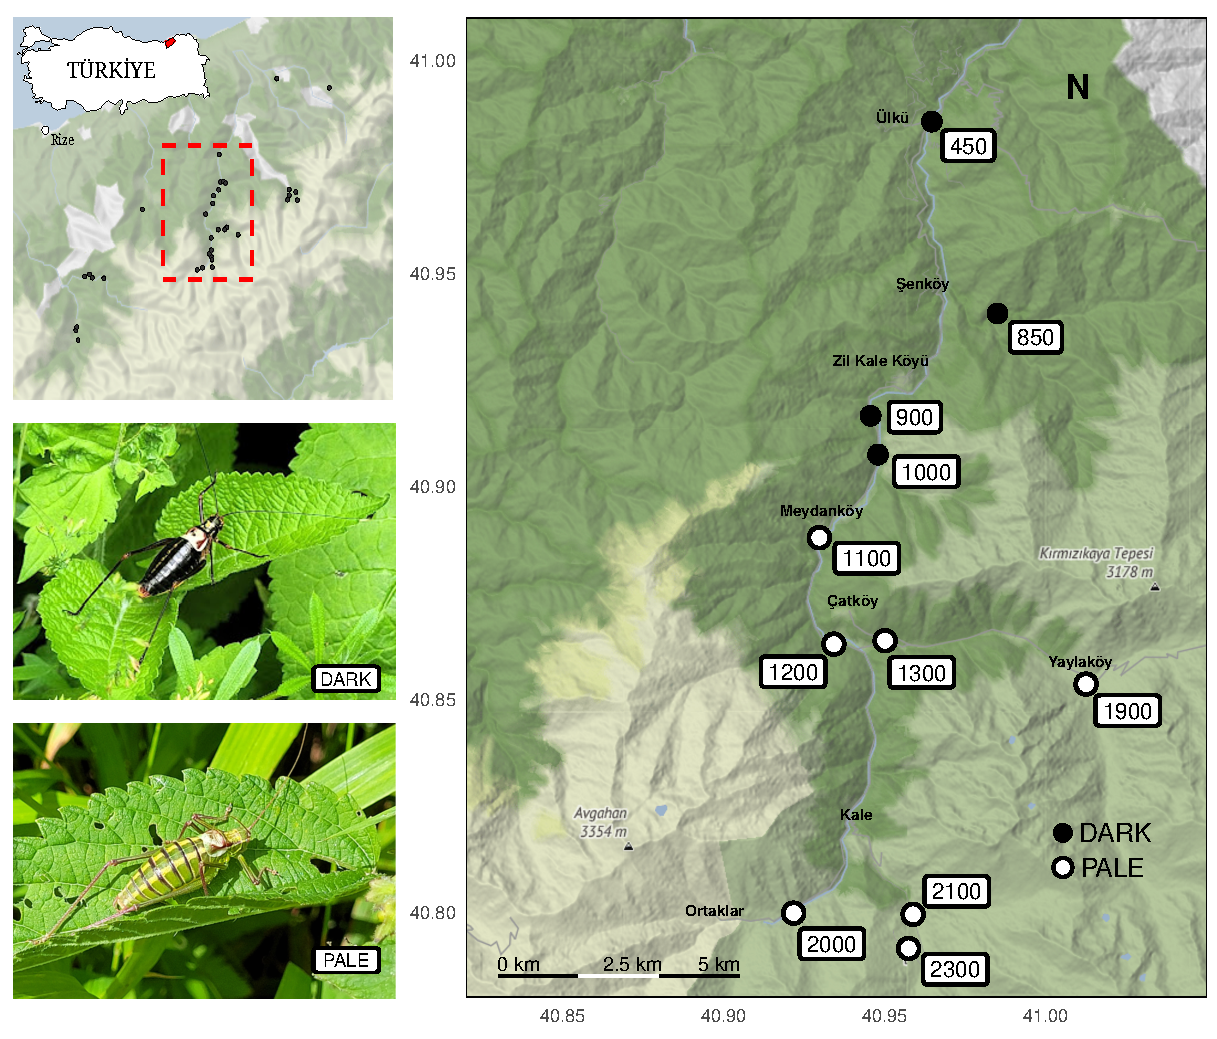
\includegraphics[width=\linewidth]{Figure_1.pdf}
\captionsetup{justification=raggedright,singlelinecheck=false,width=\linewidth, font=normalsize}
\captionof{figure}{Sampling locations of \textit{I. rizeensis} in the Fırtına Valley, Türkiye. Map showing the 11 collection sites along an altitudinal gradient within the Fırtına Valley. Village names and elevation values (in meters) are indicated. Sampling locations are categorized based on the two major colour morphs of \textit{I. rizeensis} dark and pale.}
\label{fig:1}
\end{minipage}
\end{flushleft}
\end{figure}

\clearpage
\begin{figure}[ht]
\begin{flushleft}
\begin{minipage}{0.9\textwidth}
\includegraphics[width=\linewidth]{Figure_2.pdf}
\captionsetup{justification=raggedright,singlelinecheck=false,width=\linewidth, font=normalsize}
\captionof{figure}{Genetic structure and differentiation of \textit{I. rizeensis} along an alitudinal gradient in the Fırtına Valley. \textbf{(A)} Principal Component Analysis (PCA) of genetic variation, showing genetic structuring between lower-altitude (dark-colored) and higher-altitude (pale-colored) individuals along PC1. \textbf{(B)} Admixture proportions for $K=3$, illustrating distinct genetic ancestries at low (black) and high (green) altitudes, with mid-altitude populations exhibiting mixed ancestry. \textbf{(C)} Isolation-by-distance (IBD) pattern revealed by Mantel tests, showing significant patterns of genetic differentiation along the altitudinal gradient as measured by $F_{ST}$.}
\label{fig:2}
\end{minipage}
\end{flushleft}
\end{figure}

\clearpage
\begin{figure}[ht]
\begin{flushleft}
\begin{minipage}{0.8\textwidth}
\includegraphics[width=\linewidth]{Figure_3.pdf}
\captionsetup{justification=raggedright,singlelinecheck=false,width=\linewidth, font=normalsize}
\captionof{figure}{Nucleotide diversity \textbf{(A)} and genetic differentiation \textbf{(B)} for adaptive and neutral loci in \textit{I. rizeensis} along an alitudinal gradient in the Fırtına Valley.}
\label{fig:3}
\end{minipage}
\end{flushleft}
\end{figure}

\clearpage
\begin{figure}[ht]
\begin{flushleft}
\begin{minipage}{0.8\textwidth}
\includegraphics[width=\linewidth]{Figure_4.pdf}
\captionsetup{justification=raggedright,singlelinecheck=false,width=\linewidth, font=normalsize}
\captionof{figure}{Altitudinal variation in allele frequencies for the 102 SNPs significantly associated with elevation in \textit{I. rizeensis}, showing two distinct trends where the minor allele frequency either increases or decreases with altitude.}
\label{fig:4}
\end{minipage}
\end{flushleft}
\end{figure}

\clearpage
\begin{figure}[ht]
\begin{flushleft}
\begin{minipage}{0.9\textwidth}
\includegraphics[width=\linewidth]{Figure_5.pdf}
\captionsetup{justification=raggedright,singlelinecheck=false,width=\linewidth, font=normalsize}
\captionof{figure}{Genetic differentiation between dark and pale colour morphs of \textit{I. rizeensis} based on Discriminant Analysis of Principal Components (DAPC). \textbf{(A)} DAPC density plot along Discriminant Function 1 (DF1), showing clear separation between the morphs. \textbf{(B)} SNP loadings on DF1 identifying three major-effect loci contributing to morph differentiation. \textbf{(C)} Genotypic states at the three major loci along the altitudinal gradient. HMJ = Homozygote Major; HT = Heterozygote; HMN = Homozygote Minor.}
\label{fig:5}
\end{minipage}
\end{flushleft}
\end{figure}

\end{document}